\section{Market-Event Case Studies}
\label{app:market_events}

This appendix examines key market events from 2020 to 2026 using the thesis's main variable: the rolling Pearson correlation between Bitcoin and traditional assets. The main timeline and correlation regime map first summarise all eleven events. This is followed by a detailed analysis of four representative events: the COVID crash, the FTX collapse, the SVB banking crisis, and the 2025 ``Liberation Day'' tariff shock. These events were selected to cover the main types of regimes: a liquidity-driven co-crash, a crypto-specific shock, a brief safe-haven decoupling, and a macro risk-off shock. The remaining seven events are marked on the main timeline and are fully reproduced in the 08\_Market\_Events\_Showcase.ipynb notebook in the repository. The goal is to link the quantitative results from Chapter~4 to specific historical events and to show how the regime-transition problem appears in practice.

% ─────────────────────────────────────────────────────────────────────────────
\subsection*{Master Timeline}

Figure~\ref{fig:events_timeline} shows the full sample period with all eleven events marked. The three panels display Bitcoin's normalised price trajectory on a logarithmic scale, the S\&P~500 and NASDAQ together with gold, and the 30-day rolling Pearson correlation between BTC and the S\&P~500. The event markers show how correlation spikes cluster around macro risk-off episodes while remaining subdued during crypto-specific events.

\begin{figure}[H]
    \centering
    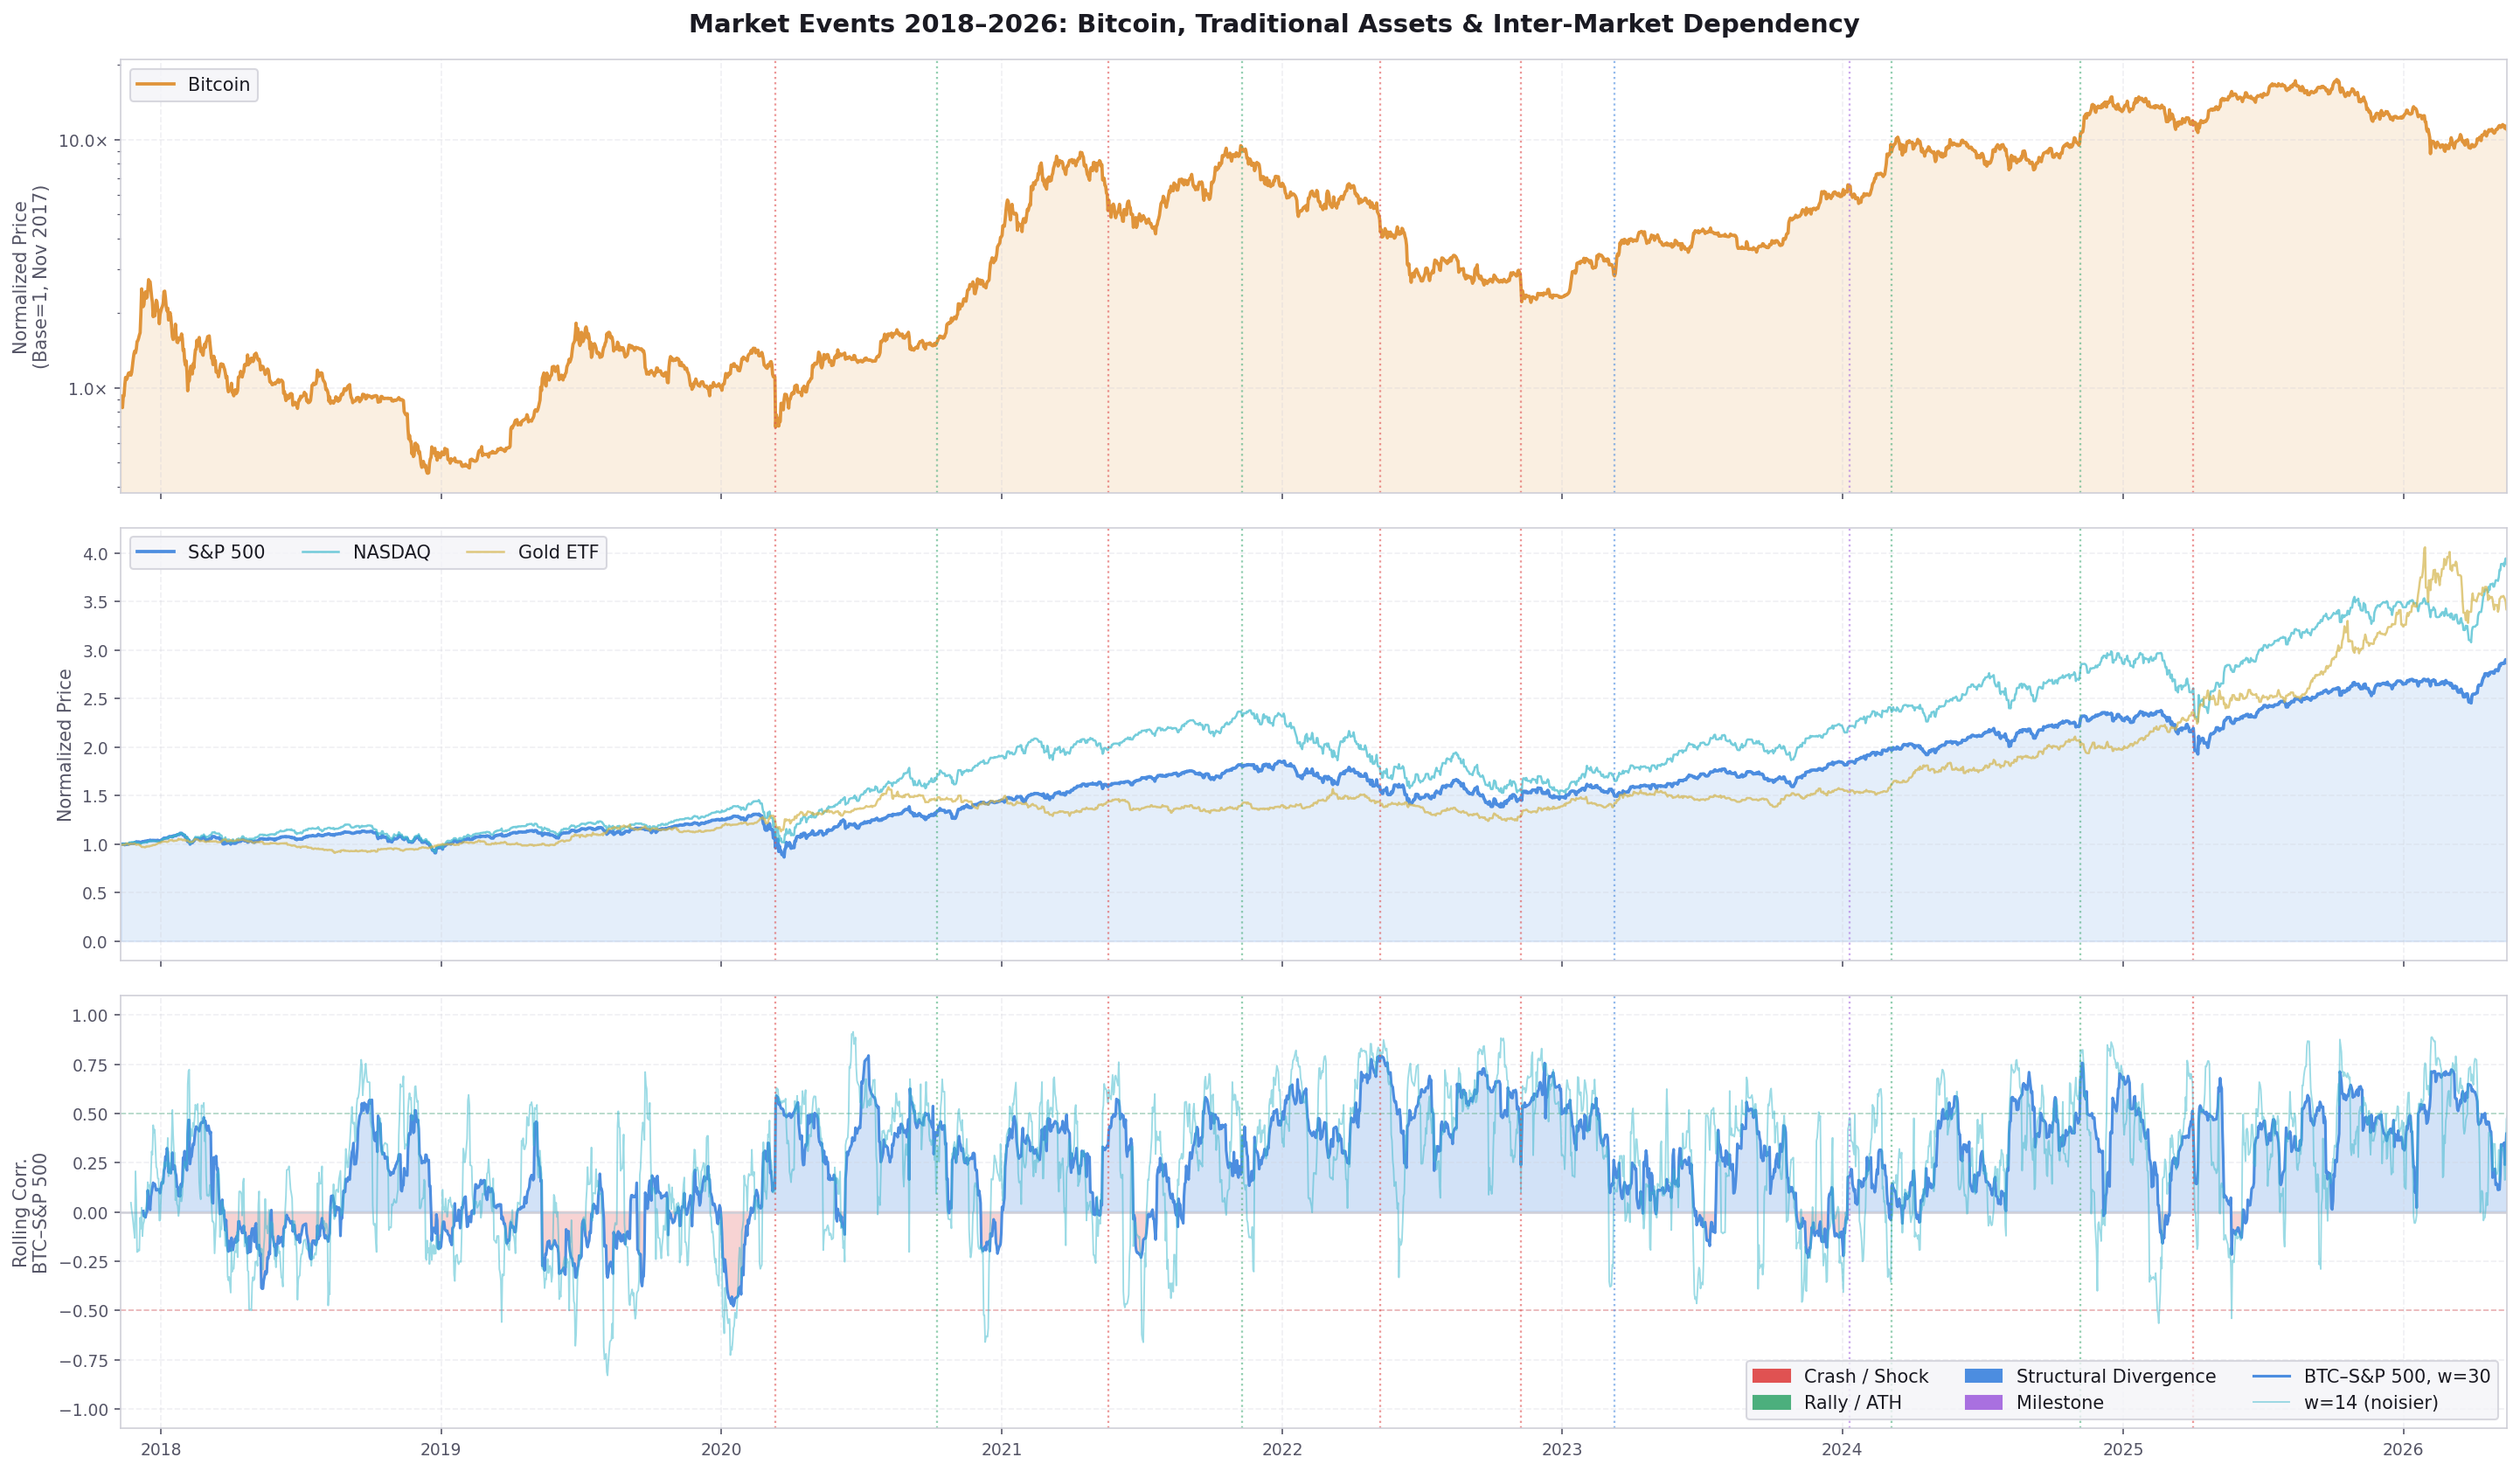
\includegraphics[width=\textwidth]{../outputs/figures/market_events_master_timeline.png}
    \caption{Master timeline 2018--2026: Bitcoin price, conventional-asset prices,
             and the 30-day rolling BTC--S\&P~500 correlation, with all eleven
             landmark events marked. Red dotted lines~=~crash/shock events;
             green~=~rallies and all-time highs; blue~=~structural divergences;
             purple~=~institutional milestones.}
    \label{fig:events_timeline}
\end{figure}

% ─────────────────────────────────────────────────────────────────────────────
\subsection*{Correlation Regime Map}

Figure~\ref{fig:events_heatmap} summarises all events jointly.
The left panel shows the 30-day average BTC correlation with each conventional asset
\emph{after} each event; the right panel shows the change in correlation
($\Delta\rho = \text{post} - \text{pre}$), isolating the regime shift associated
with the event itself.

\begin{figure}[H]
    \centering
    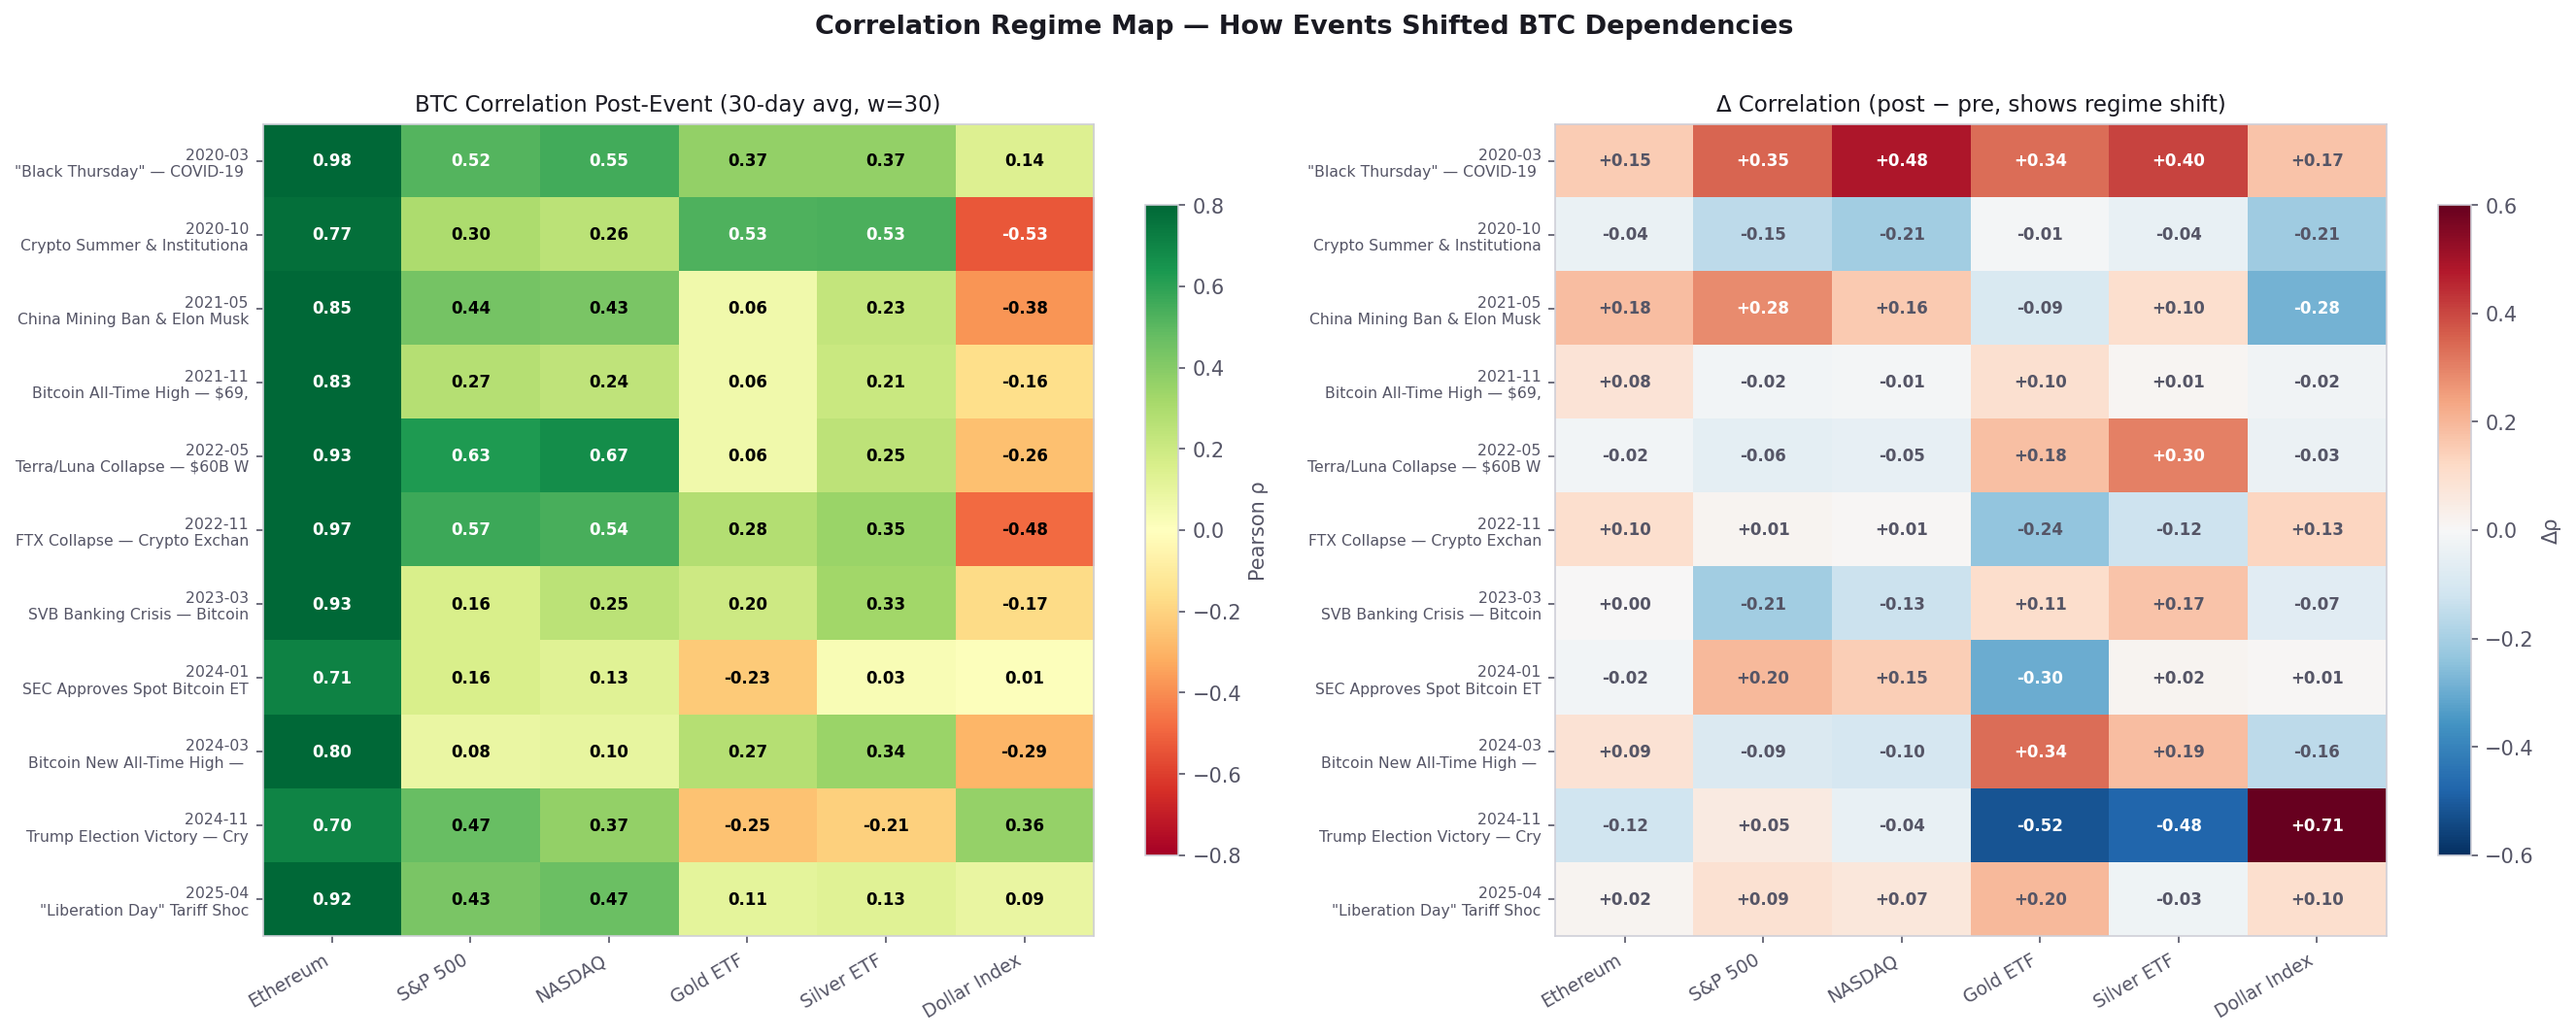
\includegraphics[width=\textwidth]{../outputs/figures/market_events_correlation_heatmap.png}
    \caption{Correlation regime map. Left: post-event BTC correlation (30-day average)
             with each conventional asset. Right: change in correlation relative to
             the 30-day pre-event average. Red/blue = strong positive/negative shifts.}
    \label{fig:events_heatmap}
\end{figure}

% ─────────────────────────────────────────────────────────────────────────────
\subsection*{Individual Event Panels}

The following figures provide a four-panel deep-dive for each of the four
representative events: (top-left) normalised price trajectories for Bitcoin and the
most relevant comparison assets; (top-right) daily log-returns as a bar chart;
(bottom-left) 30-day and 14-day rolling BTC correlation with the primary comparison
asset; (bottom-right) pre-/post-event correlation for all pairs.

\paragraph{Event 1 --- COVID Black Thursday (12 March 2020).}
Bitcoin fell about 37\% in a single session, sharply outpacing the S\&P~500's 10\% drop. The 30-day BTC--S\&P~500 correlation rose from about 0.17 to about 0.52. This was a liquidity-driven sell-off, in which Bitcoin's diversification benefit temporarily disappeared: with margin calls forcing simultaneous liquidation across asset classes, the usual distinctions between them stopped mattering. Figure~\ref{fig:event_covid} shows the episode.

\needspace{4\baselineskip}
\begin{figure}[H]
    \centering
    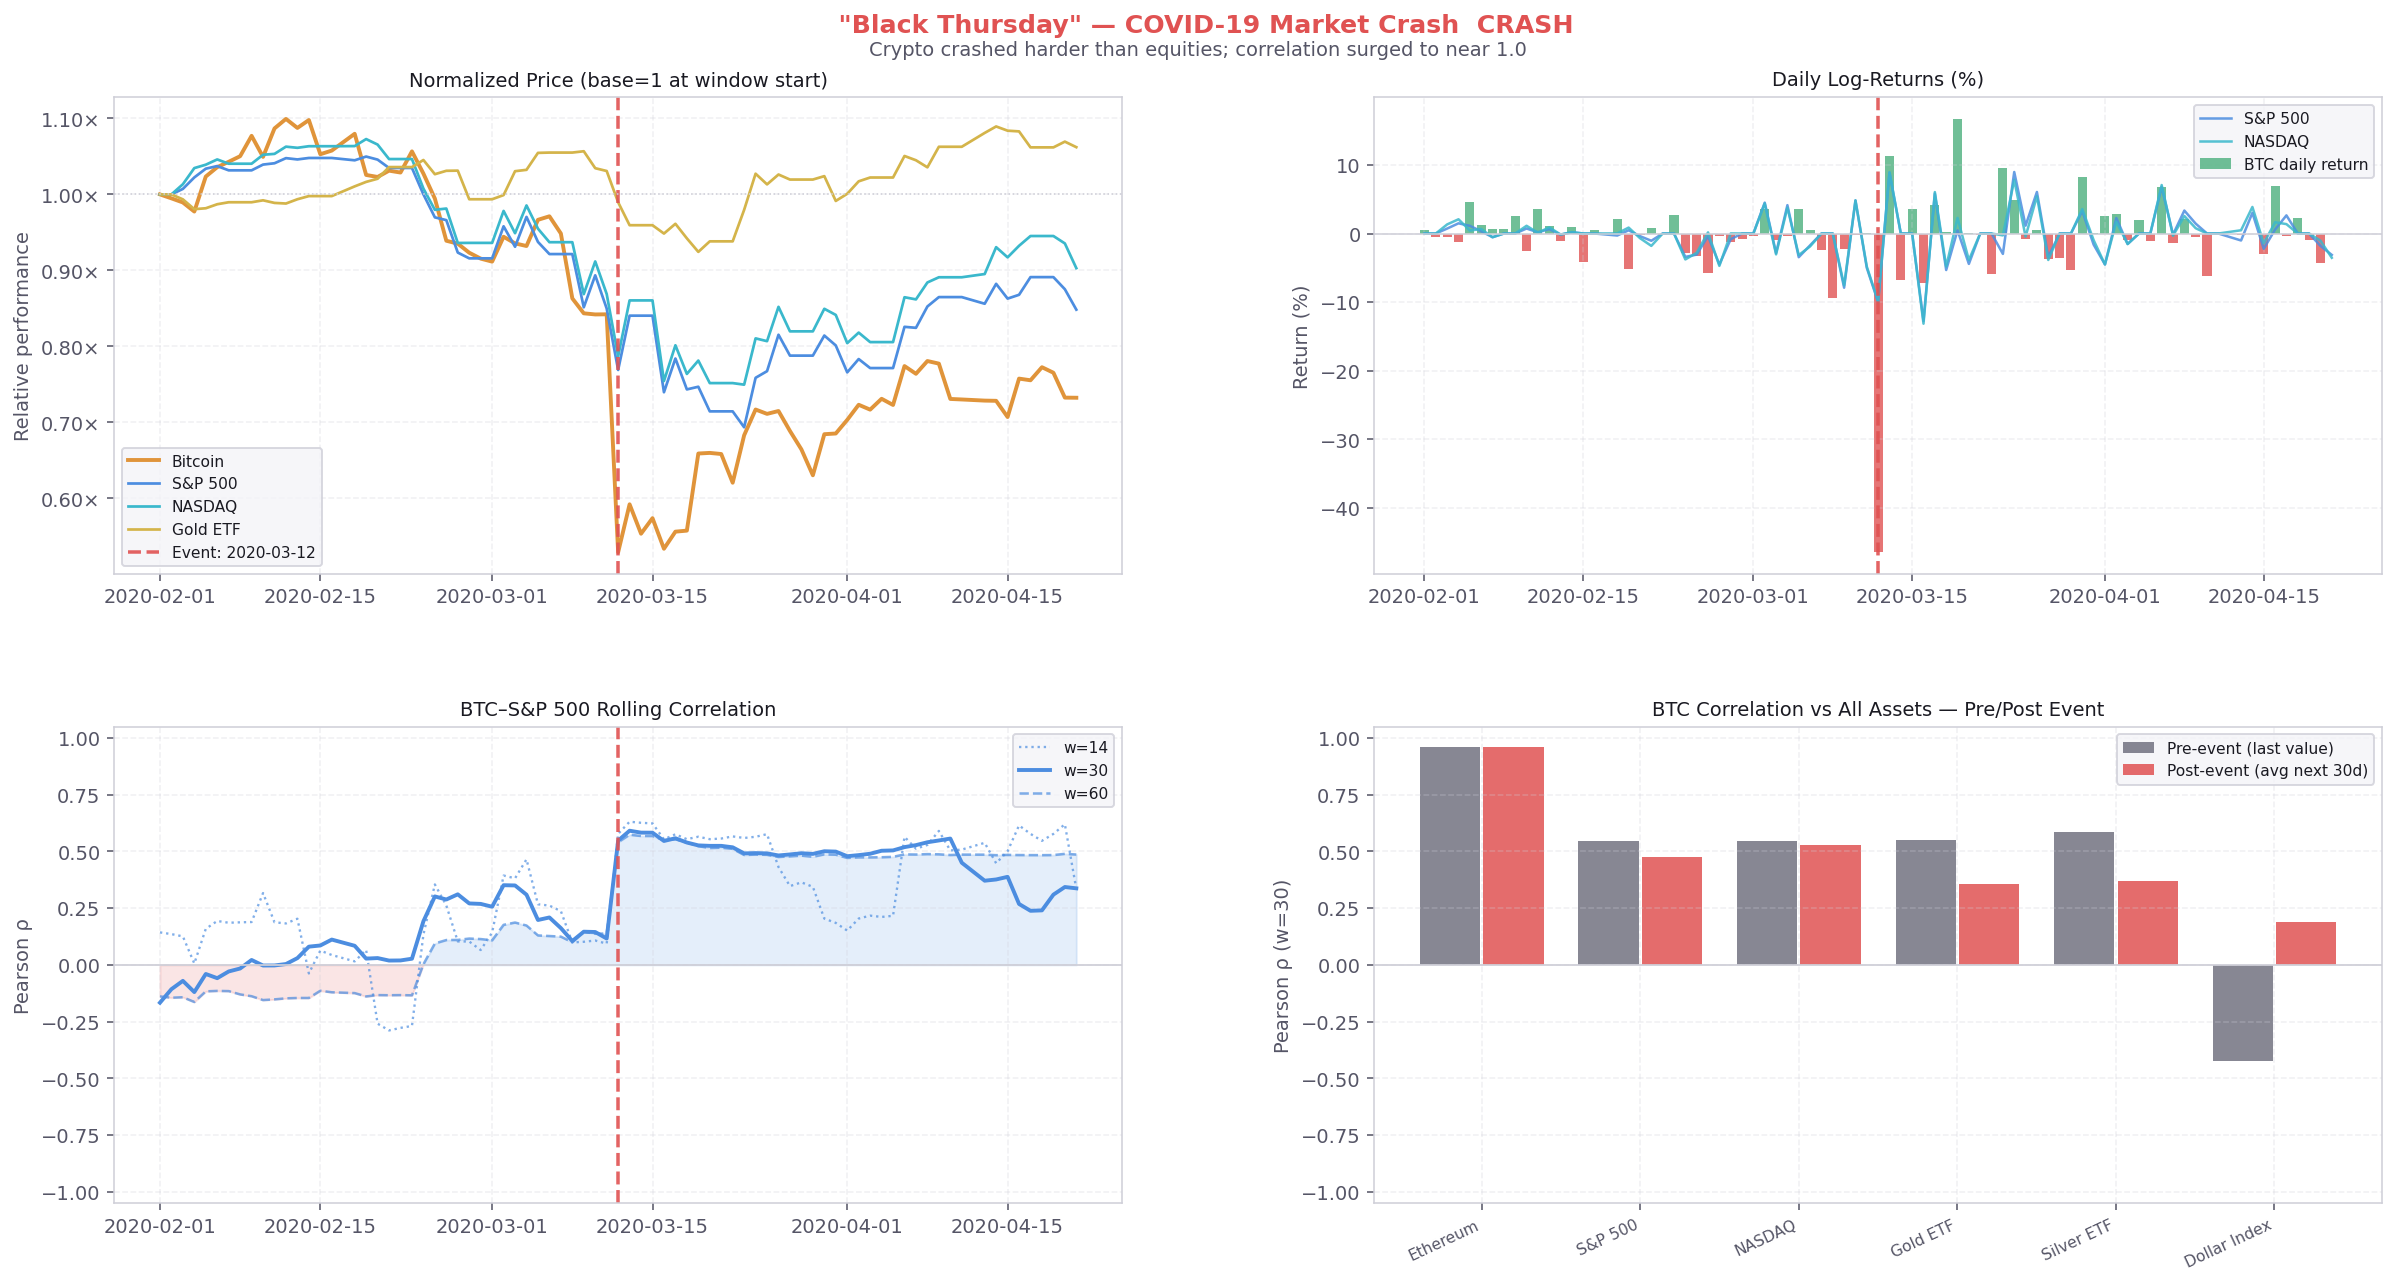
\includegraphics[width=\textwidth]{../outputs/figures/event_covid.png}
    \caption{Event 1 --- COVID Black Thursday, 12 March 2020. Source: \protect\href{https://www.reuters.com/article/us-health-coronavirus-markets-idUSKBN20Z0TO}{Reuters}.}
    \label{fig:event_covid}
\end{figure}

\paragraph{Event 2 --- FTX Collapse (8--11 November 2022).}
The exchange filed for bankruptcy and Bitcoin fell about 25\% over the following two weeks. The S\&P~500 \emph{rose} that same week on a positive CPI print, producing a sharp short-term decoupling: the 14-day BTC--equity correlation fell from about 0.6 toward zero, while the 30-day measure barely moved (about 0.55). The contrast between the two window lengths is the point of the episode. A shock confined to the crypto market registers immediately in the short window and is almost invisible in the longer one, which is exactly the trade-off between responsiveness and smoothness discussed in Section~\ref{sec:window_sensitivity}. Figure~\ref{fig:event_ftx} shows the episode.

\begin{figure}[H]
    \centering
    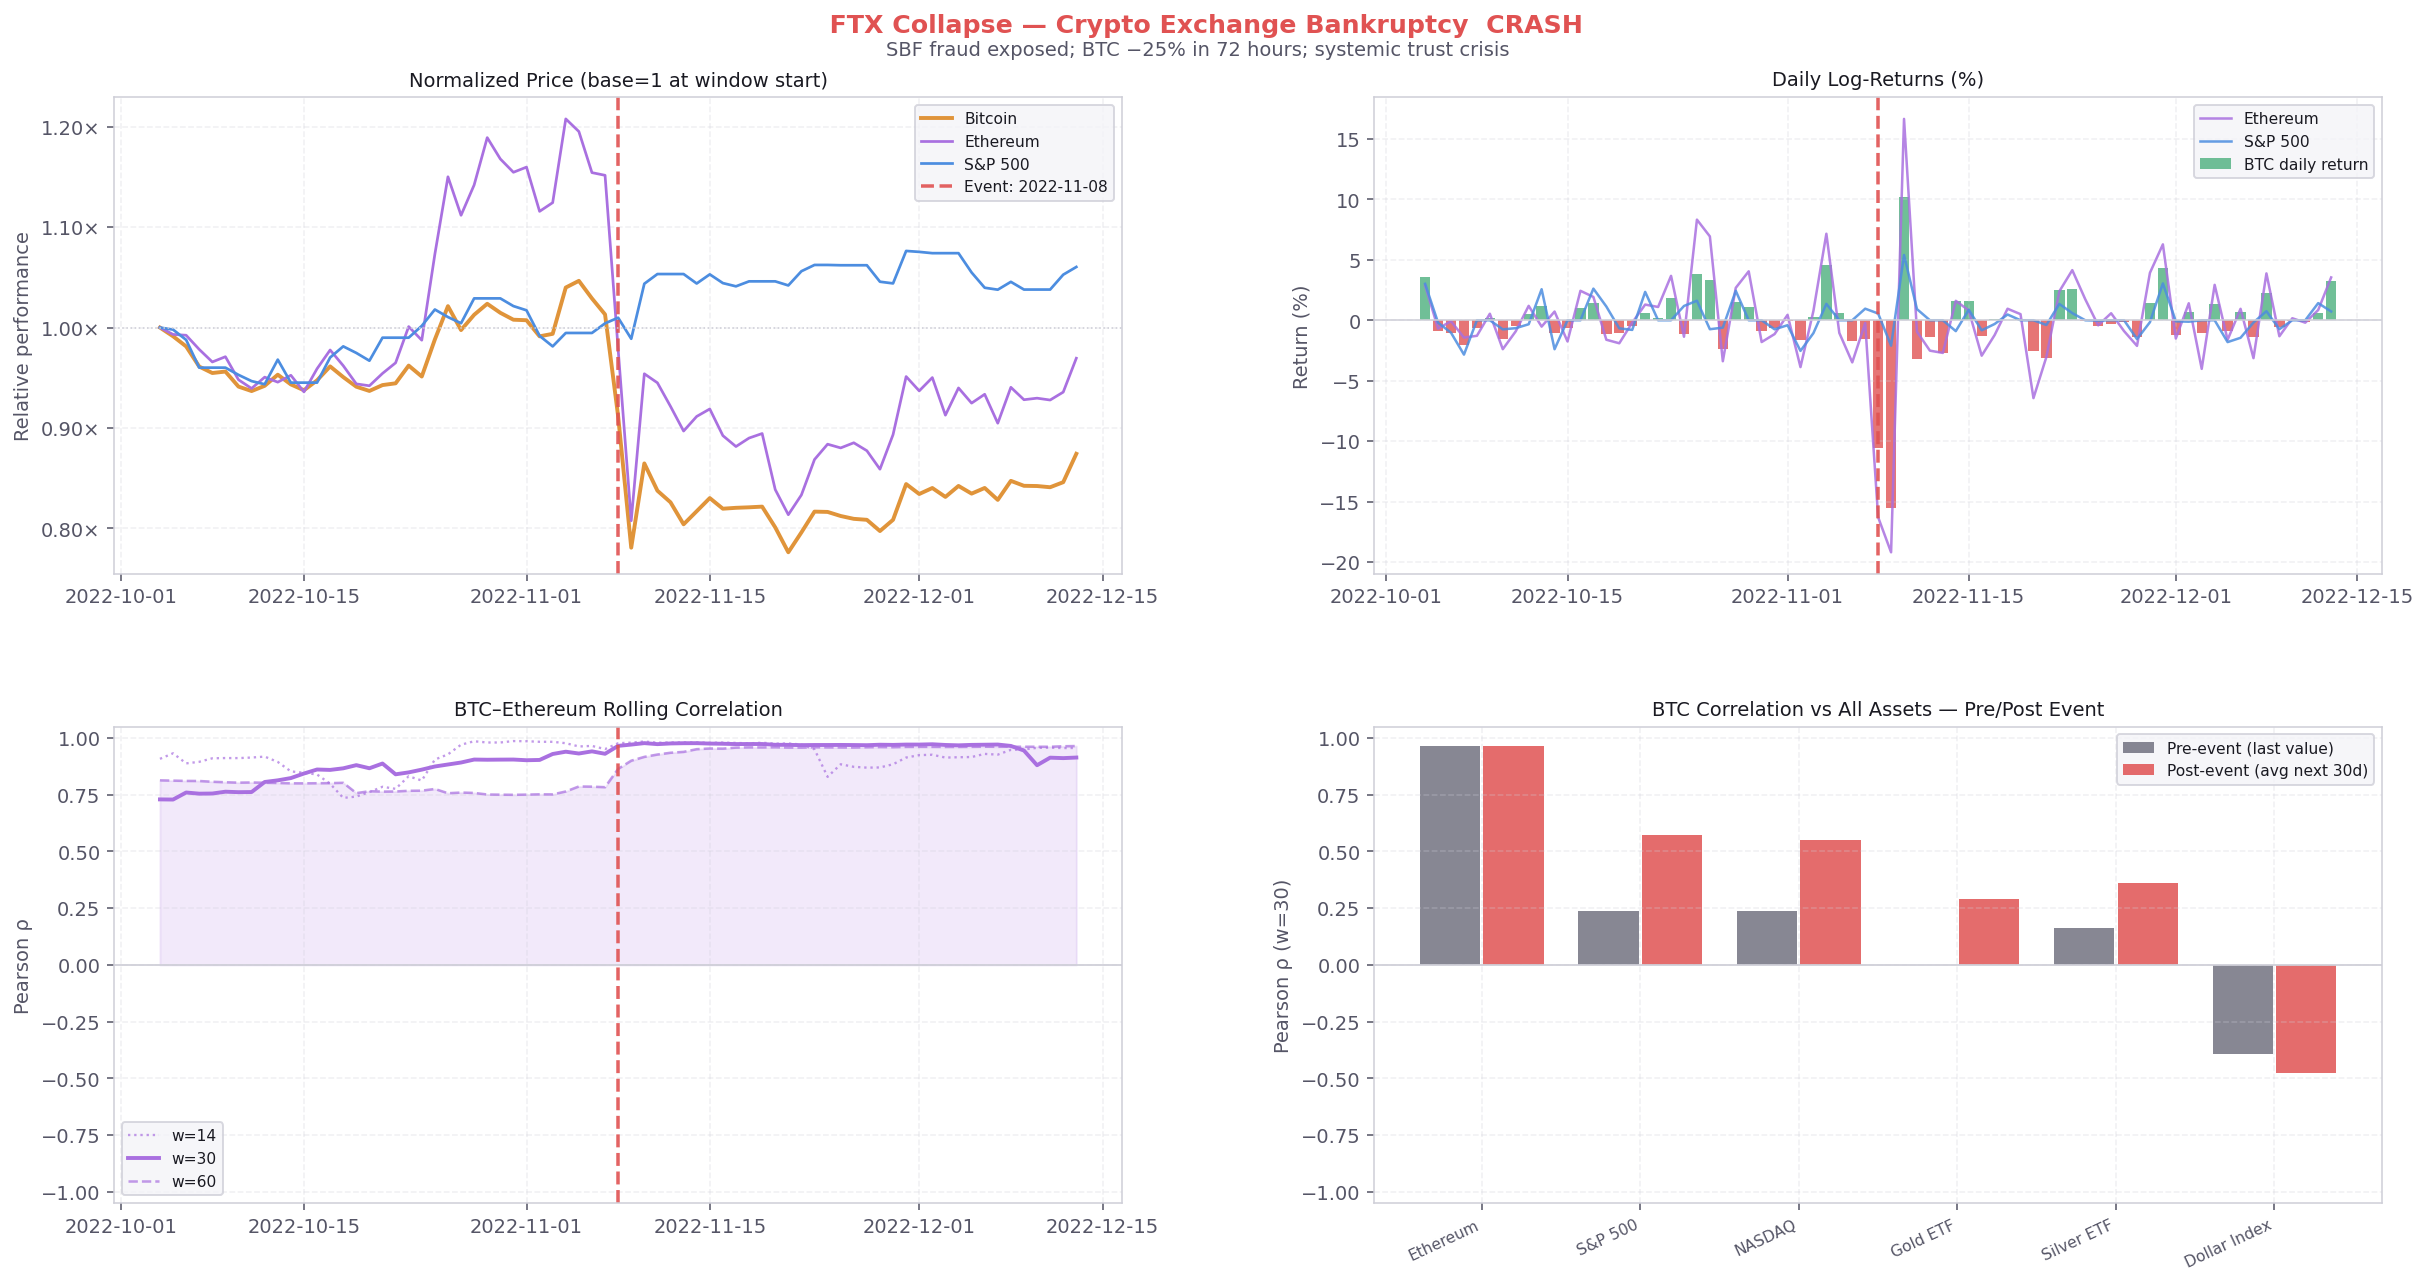
\includegraphics[width=\textwidth]{../outputs/figures/event_ftx.png}
    \caption{Event 2 --- FTX collapse, 8--11 November 2022. Source: \protect\href{https://www.bbc.com/news/technology-63631492}{BBC News}.}
    \label{fig:event_ftx}
\end{figure}

\paragraph{Event 3 --- SVB Banking Crisis (10 March 2023).}
Silicon Valley Bank's failure triggered a Bitcoin rally of about 40\% over the following week as investors sought alternatives to the banking system. Both Bitcoin and gold rose (gold about 8\%) while equities fell. This is one of the rare episodes in the sample where the short-window correlation turned negative: the 14-day BTC--S\&P~500 measure dipped to about $-0.4$, while the 30-day measure fell from 0.37 to 0.16. It is also the only one of the four events in which Bitcoin behaved as the safe-haven asset rather than the risk asset. Figure~\ref{fig:event_svb} shows the episode.

\begin{figure}[H]
    \centering
    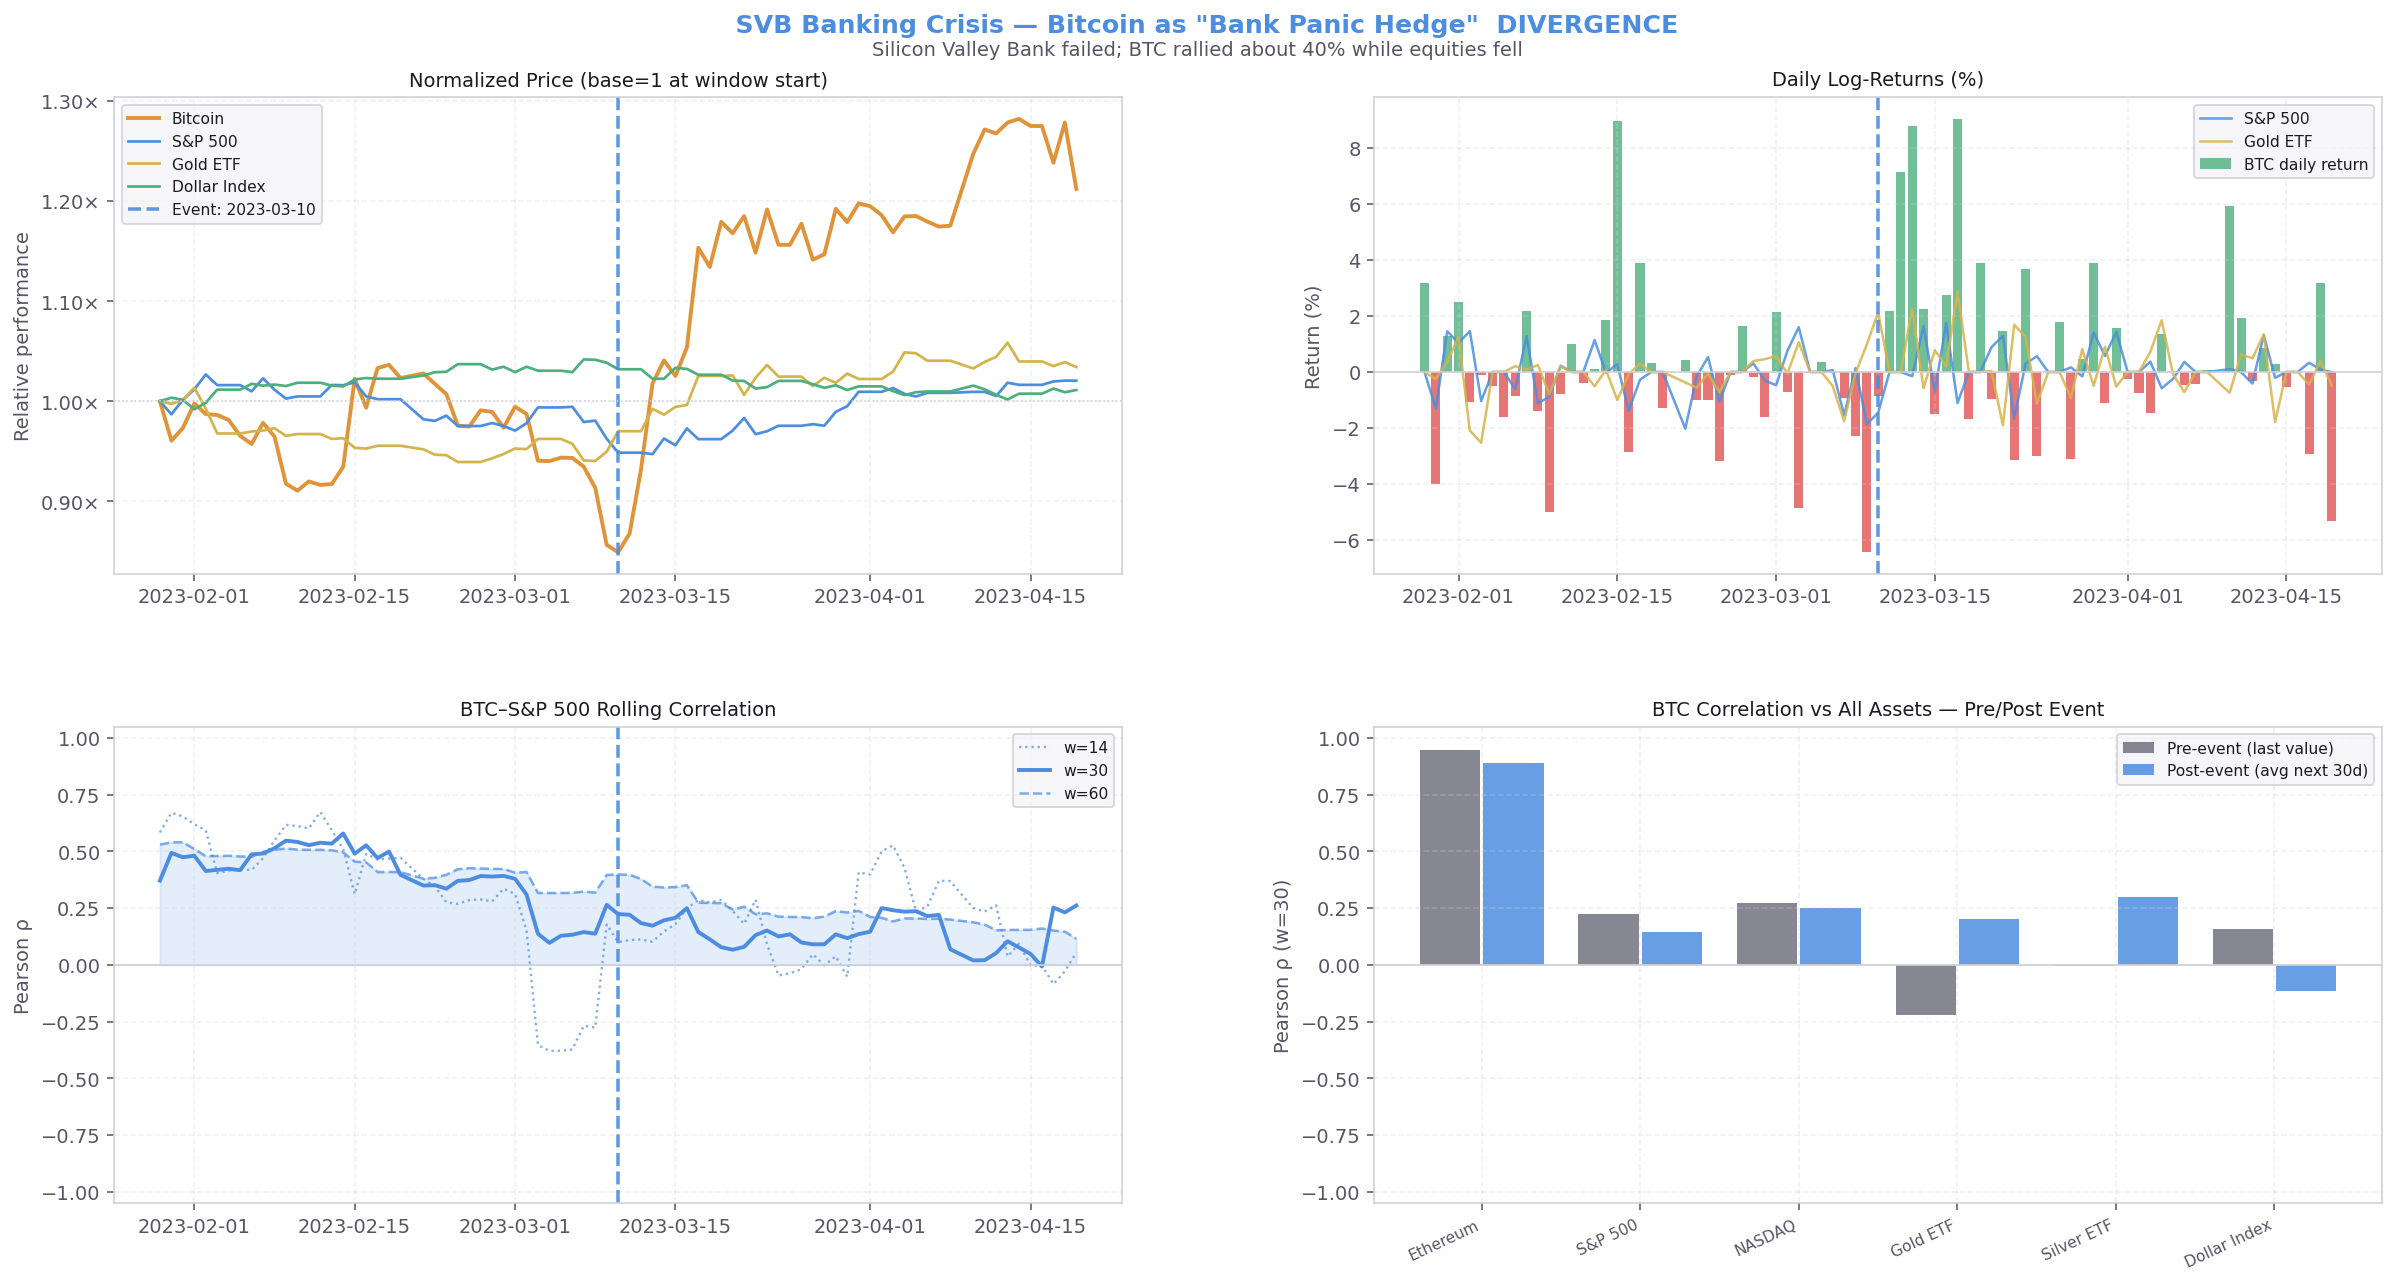
\includegraphics[width=\textwidth]{../outputs/figures/event_svb.png}
    \caption{Event 3 --- SVB banking crisis, 10 March 2023. Source: \protect\href{https://www.nytimes.com/2023/03/10/business/silicon-valley-bank-failure-explained.html}{The New York Times}.}
    \label{fig:event_svb}
\end{figure}

\paragraph{Event 4 --- ``Liberation Day'' Tariff Shock (2 April 2025).}
Sweeping tariffs on 185 countries caused the S\&P~500 to fall about 12\% in four trading days, its fastest drop since March 2020. Bitcoin fell alongside equities over the same week, while gold climbed to record highs above \$3\,000/oz. Both risk assets sold off together, confirming that Bitcoin behaves as a risk asset rather than a safe haven during acute macro shocks; even so, the 30-day rolling BTC--S\&P~500 correlation showed no clear spike, edging only from about 0.33 to 0.43, because the sharp partial recovery in the days that followed desynchronised the daily moves. The episode illustrates that even a major macro shock need not durably raise the rolling dependency, which is the main reason a correlation-based warning layer cannot be expected to fire reliably on macro events. Figure~\ref{fig:event_liberation} shows the episode.

\begin{figure}[H]
    \centering
    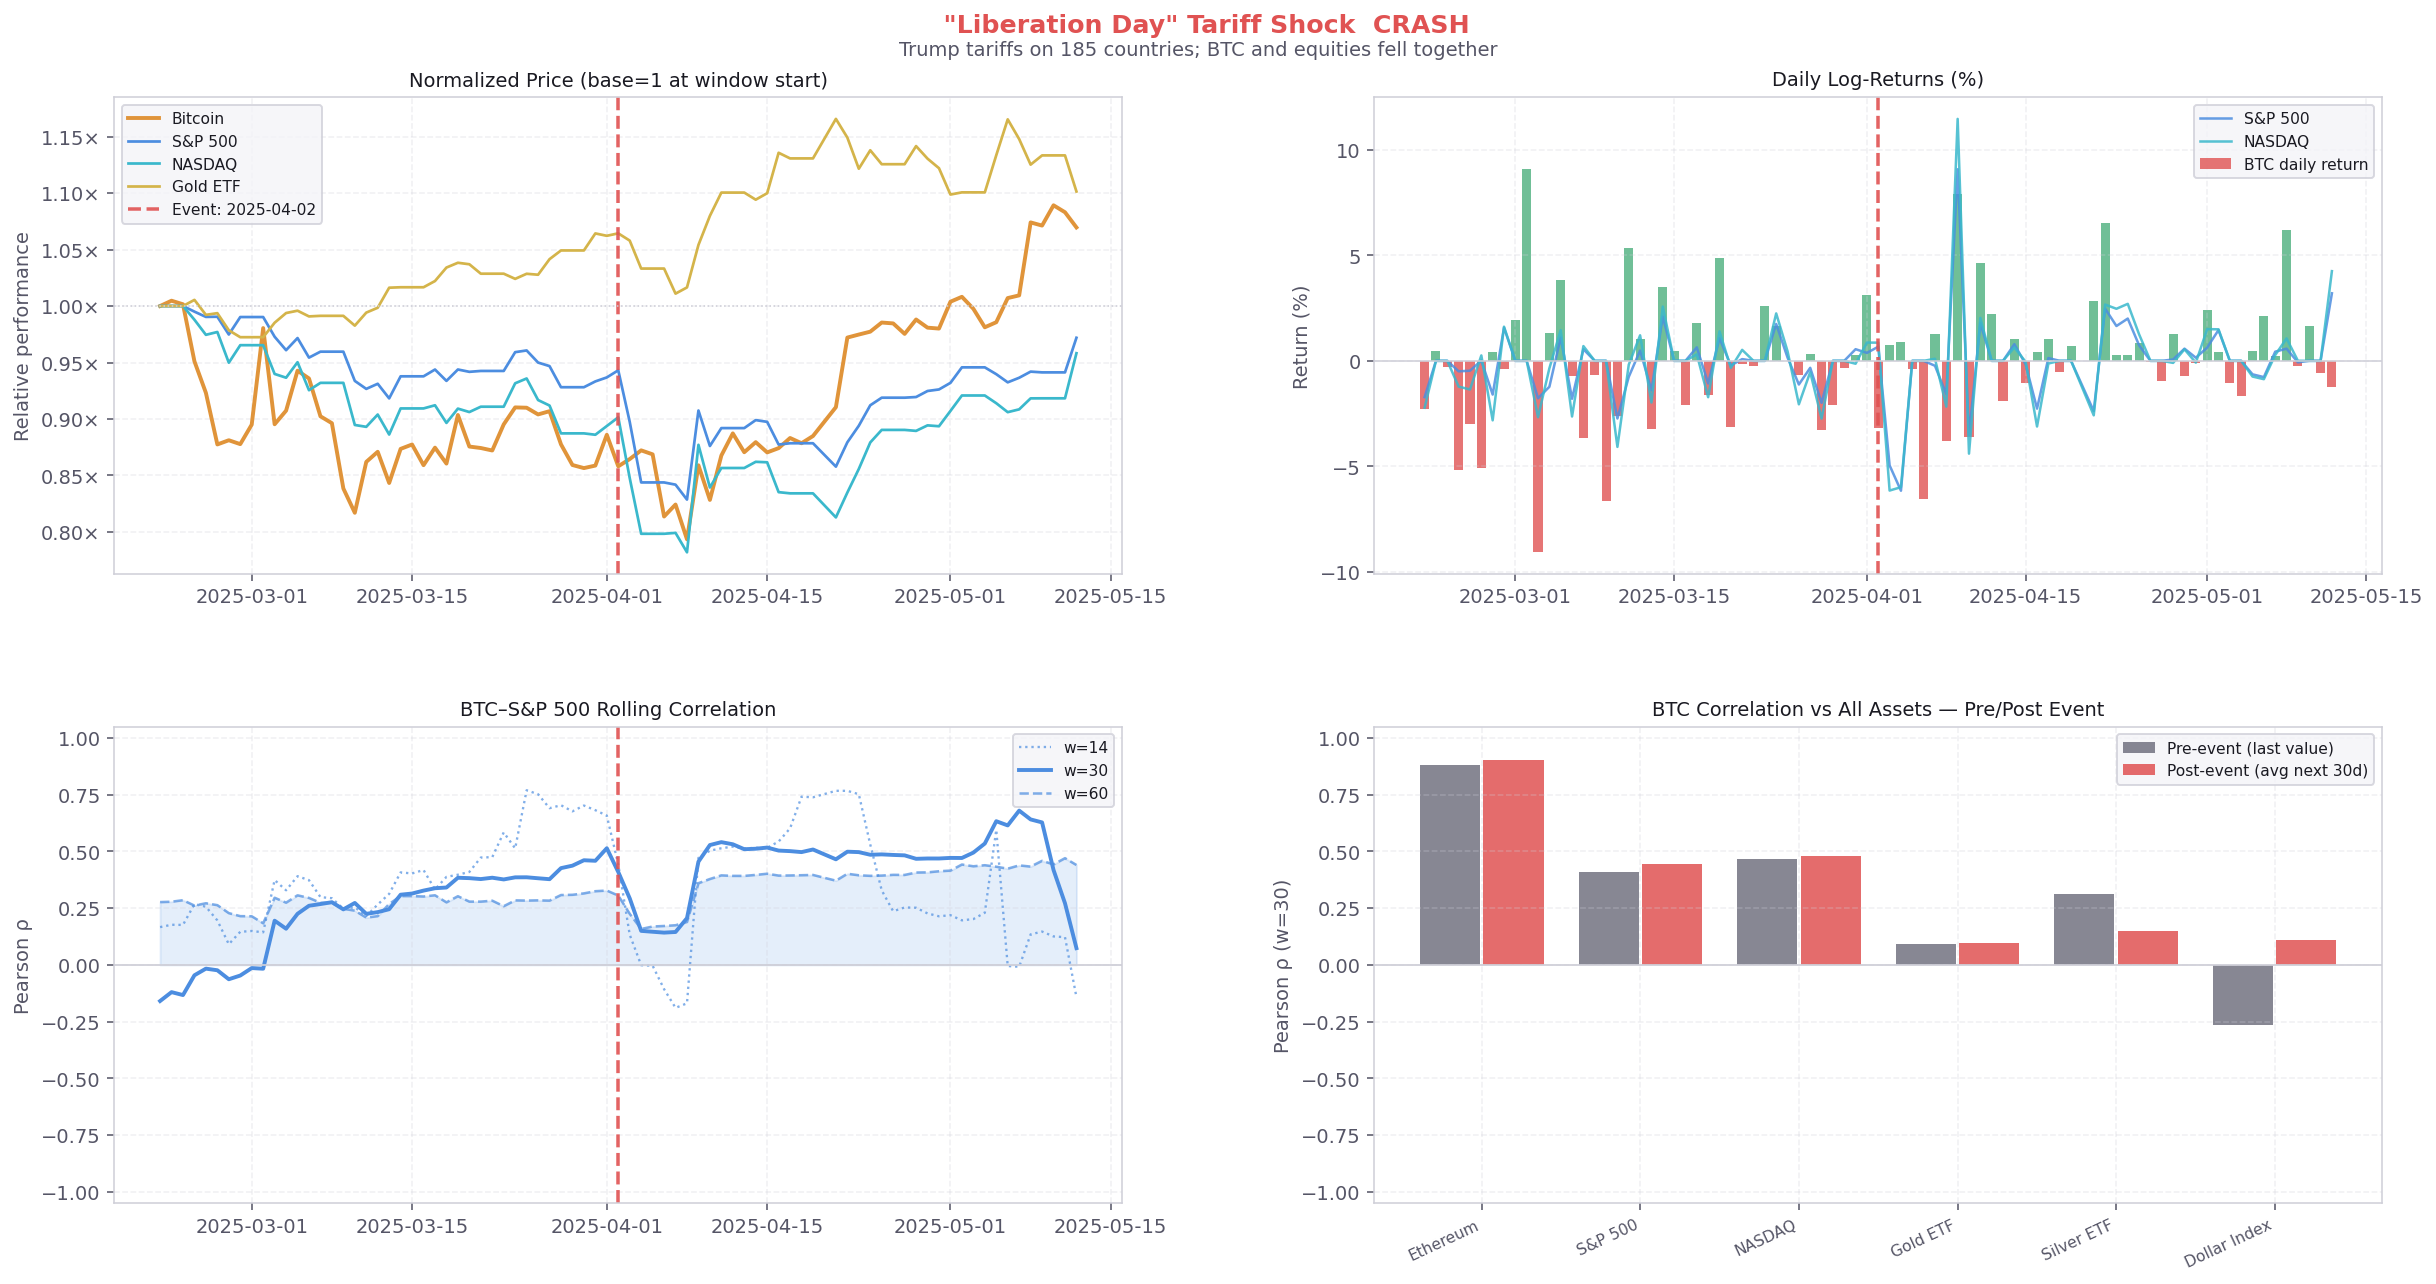
\includegraphics[width=\textwidth]{../outputs/figures/event_liberation_day.png}
    \caption{Event 4 --- ``Liberation Day'' tariff shock, 2 April 2025. Source: \protect\href{https://www.reuters.com/markets/trump-liberation-day-tariffs-global-markets-crash-2025-04-02/}{Reuters}.}
    \label{fig:event_liberation}
\end{figure}

% ─────────────────────────────────────────────────────────────────────────────
\subsection*{Interpretation}

Across the set of episodes described above and others highlighted in the main timeline, four key findings complement the overall quantitative results obtained in Chapter~4.

\begin{enumerate}
    \item Macro risk-off events lead to the largest spikes in correlation. The COVID crash in 2020 and the Fed's tightening cycle from 2021 to 2022 led to the BTC--equity correlation reaching the highest sustained levels in the sample. The 30-day indicator rose to about 0.52 in March 2020 and remained at 0.6--0.7 during the 2022 selloff. Figure~\ref{fig:rolling_rmse} also shows the periods when the rolling RMSE reaches its maximum. In contrast, the shock caused by Liberation Day in 2025 was accompanied by a sharp drop in prices, but the sliding correlation remained virtually unchanged. This shows that even severe macroeconomic shocks do not always increase the measurable dependence.

    \item Due to the shocks associated with cryptocurrencies, equity correlations often remain virtually unchanged. The ban on mining in China, the collapse of Luna and the bankruptcy of FTX led to large losses of bitcoin, while the stock markets remained virtually unchanged. These events led to only small and temporary changes in the dynamic correlation and did not lead to long-term shifts in the relationship.

    \item The institutional era that has come since 2024 has led to increased correlation. After the approval of the ETF in January 2024, institutional capital began to flow into bitcoin through the ETF products. This means that bitcoin is increasingly trading under the same risk-on/risk-off frameworks as growth equities. Thus, the 30-day BTC--NASDAQ correlation remains at a high level, averaging about 0.36 from 2024 to 2026. However, it has not yet reached the peak of 0.58, which was observed during the monetary policy tightening cycle in 2022, when both assets were sold off at the same time.

    \item Safe-haven episodes do happen, but they are short-lived. The SVB crisis led to a genuinely negative correlation between BTC and equity, but it lasted only two to three weeks before it returned to normal. Such a short duration helps explain why persistence-based models continue to dominate out-of-sample: the autoregression signal is strong enough to absorb regime shifts after a short delay, even if it cannot anticipate them.
\end{enumerate}

A complete set of event level data, summary statistics, and news links for all eleven episodes are automatically generated by notebook 08\_Market\_Events\_Showcase.ipynb, which is launched as the final step of \texttt{run\_all.py}.

\clearpage
